\documentclass[10pt,twocolumn]{article} 

\usepackage{graphicx}
\usepackage{amssymb,amsmath,epsfig,color} 
\usepackage{rotating} 
\usepackage{geometry,wasysym}   
\usepackage{natbib,url} 
%\usepackage{setspace}
\usepackage{listings}
\lstset{ basicstyle=\ttfamily, columns=fullflexible, frame=single, }
\usepackage[export]{adjustbox} 
\lstdefinelanguage{json}{morestring=[b]", morestring=[d]'}

\usepackage{algorithm,mdframed}
\usepackage{algorithmic}

\geometry{hmargin=2cm, vmargin=2cm}  
\setlength{\columnsep}{8mm}  
%\date{} 

%\usepackage{background}
%\backgroundsetup{
%  scale=1, color=black, opacity=0.3,
%  angle=45, position=current page.south,
%  vshift=10cm, hshift=10cm,
%  contents={  \textbf{\Huge DRAFT} }
%}

\author{G. Jouvet and al\footnote{This working document intends to be submitted for publication in a model development journal. It is opened for contributions until 30 September 2024. Contributions typically include the development of modules, or the performing and reporting of numerical experiments that assess the capabilities of IGM. All contributors will be listed as co-authors of the final paper. To date, direct contributors are (listed alphabetically): Samuel Cook, Guillaume Cordonnier, Brandon Finley, Andreas Henz, Oskar Herrmann, Fabien Maussion, Jürgen Mey, Dirk Scherler, Ethan Welty. Contact \texttt{guillaume.jouvet@unil.ch} if you wish to contribute.}}
 
\begin{document}
\allowdisplaybreaks 

\title{Concepts and capabilities of the Instructed Glacier Model (IGM v2.2.1)}

\maketitle
 
\begin{abstract}
We present the concept and capabilities of IGM (https://github.com/jouvetg/igm), 
a Python-based modeling tool designed for efficiently simulating glacier evolution 
across various scales. IGM integrates ice thermomechanics, climate-driven surface 
mass balance, mass conservation, and other processes. Within IGM, the update of all physical 
model components involves a series of mathematical operations on horizontal raster grids, 
performed by the Tensorflow library. This design choice results in high parallelization 
capabilities, particularly beneficial when executed on GPU hardware. 
The most challenging aspect of parallelization within IGM is the ice flow model, 
which leverages a physics-informed convolutional neural network trained from 
high-order ice flow physics. Conversely, components like the 
positive-degree day surface mass balance or the enthalpy thermal scheme 
take advantage of pixel-wise parallelization. Beyond its computational efficiency, 
IGM offers a user-friendly coding structure and modularity to promote community 
development, an OGGM-based module for accessing the data, data assimilation through 
underlying automatic differentiation tools, and post-processing vizualization routines. 
We present a comprehensive workflow, which includes data preprocessing, 
inverse and forward modeling, and rendering of results, enabling the rapid modeling 
of any mountain glacier globally by providing its RGI ID within a few minutes. 
\end{abstract}

\section{Introduction} 

Glacier evolution models play a crucial role in reconstructing the historical behavior
of glaciers and their relationship with past climates. Additionally, they are indispensable 
for predicting how glaciers will evolve in the future and the consequent rise in sea levels
 due to climate warming \citep{pattyn2018paradigm}.
Over the last two decades, the glaciological community has dedicated substantial efforts to 
the development of these models \citep{zekollari2022ice}. 
These models are designed to encompass a wide range of 
pertinent physical processes, including ice flow, thermodynamics, subglacial hydrology, 
and their intricate interactions with various factors such as atmospheric conditions 
(e.g., climate-driven surface mass balance), the Earth's lithosphere, and the ocean 
(e.g., iceberg calving or subaquatic melting). Prominent examples of such models include 
Full-Stokes such as Elmer/Ice \citep{Gagliardini.etal.2013} for a generic
usage, high-order such that PISM \citep{Winkelmann2011}, CISM \citep{lipscomb2019description}, 
ISSM \citep{larour2012continental}, which are popular in the ice sheet modelling community,
and SIA-based such as OGGM \citep{maussion2019open} or PyGEM \citep{rounce2020glacier}, 
which were designed for global glacier modelling.
However, the increasing complexity of models based on high-order mechanics comes with 
rising computational burdens, which can only be adressed using parallel computing.

In recent years, there has been a growing interest in employing Graphics Processing Units 
(GPUs) to tackle the computational bootleneck in ice flow modeling. 
GPUs are equipped with a larger number of cores, albeit 
at slower speeds compared to Central Processing Units (CPUs). 
GPUs have the potential of overcoming previously mentioned limitations in modeling ice flow 
and achieve substantial speed improvements \citep{rass2020modelling}.
Effectively harnessing the power of GPUs hinges on the implementation of numerical methods 
that can be subdivided into numerous parallel tasks, a particularly challenging endeavor 
when dealing with the viscous behavior of ice and the underlying diffusion equations 
governing its motion. As far as our knowledge extends, two distinct approaches have
been explored to achieve this high level of parallelization. The first approach 
involves the explicit time integration of the Shallow Ice Approximation (SIA) 
\citep{vivsnjevic2020climatic}, the Second Order SIA \citep{braedstrup2014ice},
ot the Stokes model \citep{rass2020modelling}.
While programming on GPU was a relative complex task in the past, the emergence of libraries 
such as TensorFlow and PyTorch in the popular Python language opens new opportunities
for the development of efficient glacier ice flow model at relatively limited technical level.
 
Capitalizing on recent library for efficient computation on GPU and machine learning
techniques, we outline the concept and demonstrate the capability of a Python-based
glacier evolution model -- the Instructed Glacier Model \citep[IGM,][]{jouvet2022deep} -- 
which couples ice thermomechanics, surface mass balance, and mass conservation. 
The specificity of IGM is that all physical model components are updated using relatively short 
sequence of operations on horizontal raster grids performed thanks to the Tensorflow library. 
As a result, IGM operations are highly parrallelized and therefore run very efficiently on GPU. 
Model components (such as the surface mass balanceor the Enthalpy models) 
that do not involve any horizontal 
diffusion are solvable pixel-wise, and therefore can be solved in parrallel. 
In contrast, we use a Convolutional Neural Network trained to minimise the energy associated 
with high-order ice flow physics to overcome solving high-order 3D ice flow partial differential 
equations and ensure parrallization \citep{jouvet2023ice}.
Using Tensorflow to describe all operations has an other major advange for data assimilation 
as embedded automatic differentiation tools permits to access all their derivatives, and therefore
to perform model inversion at low computational efforts \citep{jouvet2023inversion}. 
Lastly, similarly to OGGM and PyGEM,
we have implemented IGM in the widely-used programming language, Python, to make it accessible 
to a large community of glaciologists and leverage the numerous Python libraries. 
Additionally, we have designed IGM in a modular fashion to facilitate community development and 
user customization of the model.

This paper is organized as follows. First, we describe the physical models taken from the 
litterature and implemented in IGM. 
Then, we describe the coding concept and the module-wise implementation of IGM.
Last, we demonstrate its capabilities by presenting some examples of applications.
 
% The IGM code, as well as examples and documentation are hosted at \url{https://github.com/jouvetg/igm}.
 
%%%%%%%%%%%%%%%%%%%%%%%%%%%%%%%%%%%%%%%%%%%%%%%%%%%%%%%%%%%%% 
 
\section{Model}   

In the following, we use the notations $b(x,y)$, $l(x,y,t)$, $s(x,y,t)$, and $h(x,y,t)$ 
to represent the glacier bedrock, lower surface, upper surface, and ice thickness. 
Here, $(x,y)$ and $t$ denote horizontal coordinates, and the time. 
We also introduce ${\bf u}(x,y,z,t) = (u_x,u_y,u_z)$ as the 3D velocity field of the ice, 
and $T(x, y, z, t)$ and $\omega(x,y,z,t)$ to represent temperature and water content, 
respectively.


\begin{figure}[!h]
\begin{center} 
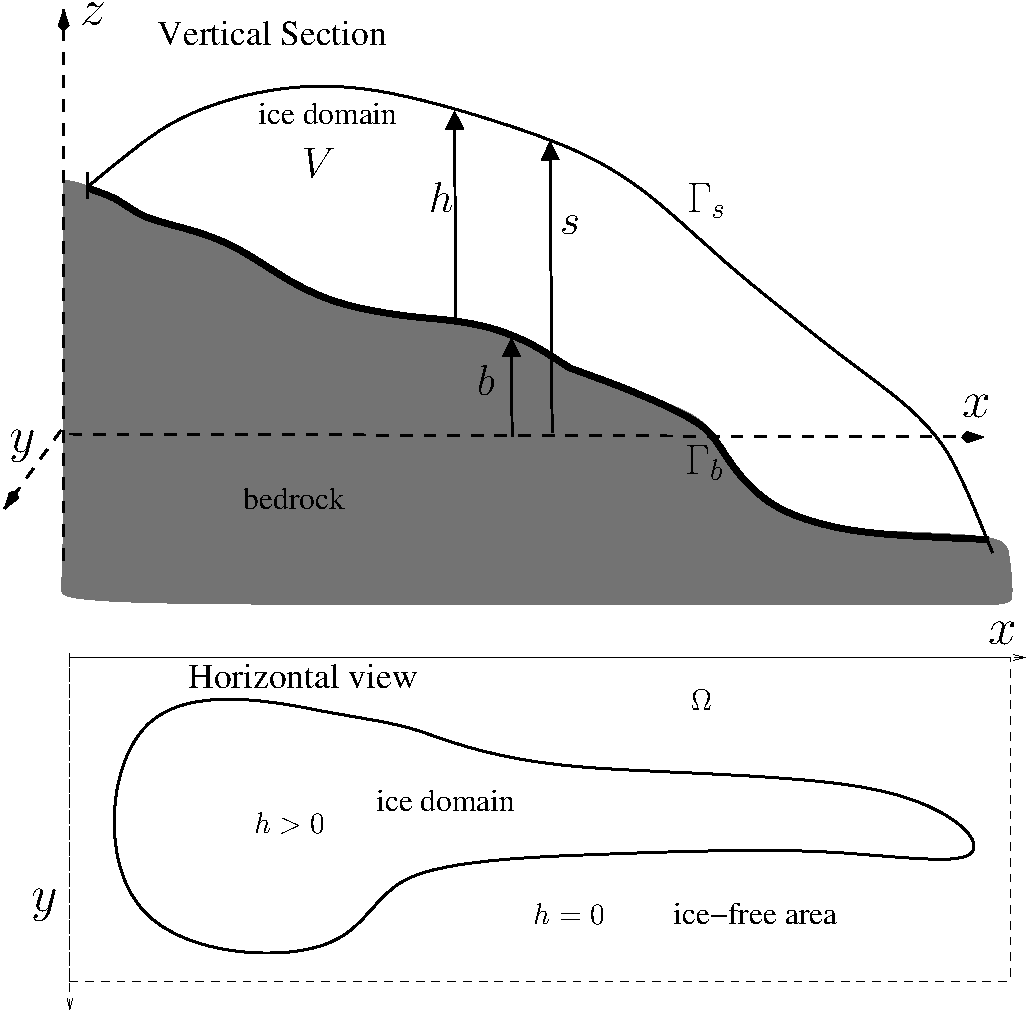
\includegraphics[width=0.48\textwidth]{fig/scheme.pdf}   
\end{center}
\caption{Cross-section and horizontal view of a glacier with notations, spatial discretization, 
main physical processes governing glacier evolution and their interactions. 
\textbf{[TODO: Include Calving Front]}
\label{notations}}
\end{figure}

\subsection{Forward modelling}

In the following sections, we describe all the physical models that are included in 
IGM and govern the evolution of the above-defined variables (Fig. \ref{notations}). 
Note that some model components (e.g. the Enthalpy and the subglacial hydrology)
may be ignored for simplicity.
These models are based on the principles of conservation of mass, momentum and energy.

\subsubsection{Mass conservation}
\label{phys_mass_conservation}

The evolution of ice thickness, denoted as $h(x, y, t)$, starting from an initial 
glacier shape, is governed by mass conservation, which connects elevation change,
ice dynamics and surface mass balance (Fig. \ref{notations}) through:
\begin{equation}
\frac{\partial h}{\partial t} + \nabla \cdot \left( \bar{\bf u} h \right) = {\rm SMB},
\label{conservationeq}
\end{equation}
where symbol $\nabla \cdot$ represents the divergence operator 
for the horizontal variables $(x, y)$, $\bar{\bf u} = (\bar{u}, \bar{v})$ denotes 
the vertically-averaged horizontal ice velocity field, while ${\rm SMB}$ represents 
the Surface Mass Balance function.

In presence of water (if $b$ lies below the water level), 
the floatation of ice is driven by Archimedes principle:
\begin{equation}
l = \max \left\{ b , - \frac{\rho}{\rho_{w}} h \right\}.
\label{floatation}
\end{equation}
where $\rho$ and $\rho_{w}$ the densities of ice and water, respectively. 
 
\subsubsection{Ice dynamics}
\label{phys_ice_dynamics}
 
The momentum conservation equation (assuming negligible inertial terms) and the 
incompressibility condition are expressed as follows:
\begin{align}
- \nabla \cdot \sigma  & =  \rho  {\bf g},  \label{eq_conservation}  \\
\nabla \cdot {\bf u}  & = 0,                   \label{eq_incomp} 
\end{align}  
where $\sigma$ is the Cauchy stress tensor, ${\bf g}= (0,0,-g)$, $g$ is the gravitational constant.
Let $\tau$ be the deviatoric stress tensor defined by 
\begin{align}
\sigma = \tau  -  p I , \label{eq_dev}  
\end{align}  
where $I$ is the identity tensor, $p$ is the pressure field, 
with the requirement that ${\rm tr} (\tau) = 0 $ so that 
$p = -(1/3) {\rm tr} (\sigma)$. Glen's flow law \citep{Glen1953}, 
which characterizes the mechanical behavior of ice, can be formulated 
as the following nonlinear relationship:
\begin{align} 
\tau & = 2 \mu {D} ({\bf u}), \label{eq_tau} 
\end{align}  
where ${D} ({\bf u})$ denotes the strain rate tensor defined by 
\begin{align} 
{D} ({\bf u}) = \frac12 ( \nabla {\bf u} +  \nabla {\bf u}^T ),
\label{def_varepsilon}  
\end{align} 
$\mu$ is the viscosity defined by 
\begin{align}  
\mu & = \frac12  A^{-\frac{1}{n}} | D ({\bf u}) |^{\frac{1}{n}-1},
\label{eq_mu}  
\end{align} 
where $ |Y|  := \sqrt{(Y : Y) / 2 }$ denotes the norm associated with the scalar product 
$(\; : \;)$ (the sum of the element-wise product), $A=A(x,y,z,t)$ is the Arrhenius factor 
and $n>1$ is the Glen's exponent.
Note that $A$ depends on the temperature of the ice \citep{Paterson1994}
\textit{via} Glen-Paterson-Budd-Lliboutry-Duval law:
\begin{align}
A(T,\omega)= A_c(T)(1+181.25 \omega), \label{defA}
\end{align}
where $A_c(T)$ is given by the Paterson-Budd law:
\begin{align}
A_c(T)= A \exp{ ( -Q / (R \, T_{pa}) )}
\end{align}
where $A$ and $Q$ have different values below and above a threshold temperature:
\begin{align}
A & = 3.985 \times 10^{-13} \, s^{-1} Pa^{-3}, & \textrm{ if } T <263.15 \, K \label{A1} \\
A & = 1.916 \times 10^3 \, s^{-1} Pa^{-3}, & \textrm{else.} \label{A2} 
\end{align}
and
\begin{align}
Q & =  60 \; {\rm kJ mol}^{-1}, & \textrm{ if } T <263.15 \, K \\
Q & = 139 \; {\rm kJ mol}^{-1}, & \textrm{else.}
\end{align}
For simplicity, we may ignore temperature dependence of $A$ for instance in the 
case the Enthalpy (Section \ref{phys_enthalpy}) is not modelled.
 
Equations \eqref{eq_conservation} to \eqref{eq_mu} describe a Stokes problem in which 
the unknowns are the 3D velocity field ${\bf u}$ and the pressure field $p$. 
To simplify the problem, we make the "hydrostatic assumption" as described by  \citep{Blatter1995}
and neglect second-order terms in the aspect ratio of the ice domain (thickness versus length) 
within the strain rate tensor $D({\bf u})$. By doing so and invoking the incompressibility equation, 
both the vertical velocity components $u_z$ and the pressure $p$ are eliminated from the 
momentum conservation equation.
The resulting model, commonly referred to as the Blatter-Pattyn model
\citep{Blatter1995}, conveniently transforms into a 3D nonlinear elliptic equation solely 
for the horizontal velocity components. This modification makes it easier to solve compared 
to the original Stokes model.

The boundary conditions that supplement \eqref{eq_conservation}, \eqref{eq_incomp} 
are the following. Stress free force applies to the ice-air interface,
\begin{equation}
\sigma \cdot {\bf n} = 0, \quad p = 0,  \label{BC_FS}
\end{equation}
where ${\bf n}$
is an outer normal vector along the surface. Along the lower surface interface, 
the nonlinear Weertman friction condition \citep[e.g.,][]{SchoofHewitt2013}
relates the basal shear stress $\tau_b$ to the sliding velocity ${\bf u}_b$ as follows:
\begin{align}
{\bf u} \cdot {\bf n} &= 0,  \label{BC_slip1} \\ 
\tau_b & = -  c |{\bf u}_b|^{m-1} {\bf u}_b, \label{BC_slip2a}
\end{align} 
where $m>0$, $c=c(x,y) > 0$, and ${\bf n}$ is the outward normal unit vector to the bedrock.

The sliding coefficient $c$ in \eqref{BC_slip2a} is defined with the Mohr-Coulomb law
\citep{Cuffey.2010}, that involves the effective pressure in the till $N_{till}$
(Section \ref{phys_subglacial_hydrology}):
\begin{align}
c  = \tau_c u_{th}^{-m} & = N_{till} \tan(\phi) u_{th}^{-m}, 
\label{sliding_param}
\end{align}
where $\phi$ is the till friction angle, and $u_{th}$ is a parameter homegenous to ice velocity
following \citet{pism-user-manual}.
In the case the Enthalpy (Section \ref{phys_enthalpy}) and the subglacial hydrology
(Section \ref{phys_subglacial_hydrology}) are not modelled, we may simply prescribe 
a constant sliding coefficient $c$, or get its spatial distribution by inverse modelling
(Section \ref{inv_model}).

Conditions on the horizontal boundaries change if there is still ice on this boundary, 
if this ice is floating, 
grounded above or below sea level \citep{Schoof2006a,Winkelmann2011}.
However, such boundary conditions can be written in a unified way:
\begin{equation}
 A^{-\frac{1}{n}}  \, h | D({\bf u}) |^{\frac{1}{n}-1} D({\bf u}) \cdot {\bf n} 
 =  \underbrace{\frac{1}{2}  \rho g 
 \left( h^2 - \frac{\rho_w}{\rho} [\min \{l,0 \}]^2 \right) {\bf n}}_{:= {\bf F}(h)},
\label{BC_SSA}
\end{equation} 
where $l$ is defined by \eqref{floatation}.
 
\subsubsection{Ice enthalpy}
\label{phys_enthalpy}

In this section, we model ice enthalpy following \citet{aschwanden2012enthalpy}.
This approach enables us to simultaneously model ice 
temperature and water content when the temperature reaches the pressure melting point, 
thereby conserving energy. Ice enthalpy influences the dynamical model in two ways: 
variations in temperature and water content lead to ice softening or hardening (Eq. \eqref{defA}), 
while enthalpy affects basal sliding conditions throught basal till water layer (Eq. \eqref{sliding_param}). 
The enthalpy, denoted as $E$, is a variable defined throughout the ice and 
is a function of both temperature, $T$, and water content, $\omega$:
\begin{align}
\label{def_enth}
E(T, \omega,p) = 
\left\{
\begin{array}{ll}
c_i (T- T_{\rm ref}), & {\rm  if } \; T < T_{\rm pmp} , \\ 
E_{\rm pmp} + L \omega, &  
{\rm if } \;  T = T_{\rm pmp},\; 0 \le \omega,
\end{array} 
\right.  
\end{align}
where $c_i$ is the heat capacity, $T_{ref}$ is a reference temperature, 
and $L$ is the latent heat of fusion. Additionally the temperature $T_{\rm pmp}$
and enthalpy $E_{\rm pmp}$ at pressure-melting point of ice are defined by   
\begin{align}
T_{\rm pmp} & = T_0 - \beta p, \label{defTpmp} \\
E_{\rm pmp} & = c_i (T_{\rm pmp}(p) - T_{\rm ref}), \label{defEpmp}
\end{align}  
where $T_0 = 273.15$ K is the melting temperature at standard pressure, and
$\beta = 7.9 \times 10^{-8}$ K Pa$^{-1}$ is the Clausius-Clapeyron constant. 

According to the definition of enthalpy provided above, we have two possible modes:
i) When the ice is cold, meaning it is below the melting point, the enthalpy is simply 
proportional to the temperature minus a reference temperature.
ii) When the ice is temperate, the enthalpy continues to increase. In this case, 
the additional component $L \omega$ accounts for the creation of water content 
through energy transfer. Therefore, one can infer the value of enthalpy, denoted as $E$, 
from both temperature, $T$, and water content, $\omega$, and \textit{vice-versa}.

The melting point temperature at pressure is adjusted for hydrostatic pressure 
$p = \rho g d$ using the following equation:
\begin{equation}
\label{Tpmp}
T_{pmp} = T_{0} - \beta \rho g d, 
\end{equation}
where $d$ represents the depth. Therefore, the "pressure-adjusted" temperature, 
denoted as $T_{pa}$, is defined as the temperature with a shift such that its 
melting point temperature reference is always zero:
$$ T_{pa} = T + \beta \rho g z. $$

The enthalpy model consists of the following advection-diffusion equation,
with horizontal diffusion being neglected:

\begin{align}
& \rho_i \left( \frac{\partial E}{ \partial t}
+ u_x \frac{\partial E}{ \partial x}
+ u_y \frac{\partial E}{ \partial y} 
+ u_z \frac{\partial E}{ \partial z} 
\right) 
 - \frac{\partial }{\partial z} \left(
K_{c,t} \frac{\partial E}{ \partial z} \right) \label{enth1} \\
& = \phi - \rho_w L D_w(\omega), \label{enth2} 
\end{align}

where $\rho_i$ is the ice density, $K_{c,t}$ equals 
$K_c = k_i/c_i$ if the ice is cold ($E<E_{pmp}$) or $K_t = \epsilon k_i/c_i$ otherwise. 
Using Glen's flow law (Eq. \eqref{eq_tau}), the strain heating $\phi$ is defined by 
\begin{equation}
\label{def_phi}
\phi = D({\bf U}) \tau = A^{-1/n} | D({\bf u}) |^{1+1/n}.
\end{equation}
The last source term $- \rho_w L D_w(\omega)$ in \eqref{enth2} permits to remove the water 
in temperate ice, $D_w(\omega)$ being a drainage function \citep{aschwanden2012enthalpy}.

At the top ice surface, the enthalpy equation is constrained by the surface temperature 
(or equivalently, the enthalpy) provided by the climate forcing, which is enforced as a 
Dirichlet condition.
At the glacier bed, there are multiple boundary conditions for the enthalpy equation
\citep{aschwanden2012enthalpy,wang2020two}:
\begin{itemize}
\item cold base and dry: $K_{c} \frac{\partial E}{ \partial z} = Q_{\rm geo} + Q_{\rm fh}$
if $E_b<E_{\rm pmp}$ and $W_{till} = 0$, 
\item cold base and wet: $ E_b = E_{\rm pmp} $ if $E_b<E_{\rm pmp}$ and $W_{till} > 0$,
\item temperate base and cold ice: $ E_b = E_{\rm pmp} $ if $E_b \ge E_{\rm pmp}$ and $W_{till}> 0$,
zero temperate basal layer,
\item temperate base, temperate ice: $ K_{t} \frac{\partial E}{ \partial z} = 0$ 
if $E_b \ge E_{\rm pmp}$ and $W_{till} > 0$, non-zero temperate basal layer,
\end{itemize}
where $Q_{\rm geo}$ and $Q_{\rm fh}$ are the geothermal heat flux, and the frictional heat flux, 
respectively. Using Weertmann law \eqref{BC_slip2a}, the latter is computed as follows:
\begin{equation}
Q_{\rm fh} = \tau_b \cdot {\bf u}_b = c | {\bf u}_b |^{m+1}. \label{def_Q}
\end{equation}
When the temperature hits the pressure-melting point at the glacier bed 
(i.e. $E \ge E_{\rm pmp}$), the basal melt rate is calculated via the following equation:
\begin{equation}
m_b = \frac{1}{\rho_i L} (Q_{fr}+Q_{geo} - K_{t,c} \frac{\partial E}{ \partial z}). 
\label{basal_melt_rate}
\end{equation}
The basal melt rate is further increased to account for the drainage of the water 
content generated throughout the entire column (last term of Eq. \eqref{enth2}).

\subsubsection{Subglacial hydrology}
\label{phys_subglacial_hydrology}

Following \citet{Bueler2015}, the basal water thickness in the till $W_{till}$ 
is computed from the basal melt rate as follows:
\begin{equation}
\frac{\partial W_{till} }{ \partial z} = \frac{m_b}{\rho_w} - C_{dr},
\label{W_till}
\end{equation}
where $C_{dr}$ is a simple drainage parameter. The till is assumed to be saturated 
when it reaches the value $W_{till}^{max} = 2$ m, therefore, the till water thickness 
is capped to this value. The effective thickness of water within the till $N_{till}$ 
is computed from the saturation ratio $s= W_{till} / W_{till}^{max}$ by the formula
\citep{Bueler2015}:
\begin{equation}
N_{till} = \min \left\{ p, N_0 \left( \frac{\delta P}{N_0} \right)^s 10^{(e_0/C_c)(1-s)} \right\},
\end{equation}
where $p$ is the ice overburden pressure and the remaining parameters are constant. 
 
\subsubsection{Surface mass balance}
\label{phys_smb}

IGM comes with several surface mass balance models.

The simplest one implements a classical
linar relation between Equilibrium Line Altitude (ELA) and altitude:
\begin{align}
SMB(z) & = \min(\beta_{acc} (z-z_{ELA}),m_{acc})\quad\textrm{if}\;z>z_{ELA}, \label{smb1} \\
SMB(z) & = \beta_{abl} (z-z_{ELA})\quad\textrm{else}, \label{smb2} 
\end{align}
where $z_{ELA}$ is the ELA, $\beta_{abl}$ and $\beta_{acc}$
are ablation and accumulation gradients, and $m_{acc}$ is the maximum surface mass balance.
 
Second, IGM incorporates a temperature index model \citep{hock2003} to calculate the 
surface mass balance based on seasonal temperature and precipitation fields.
In this model, surface accumulation equals solid precipitation when the temperature is 
below a threshold (usually $0^{\circ}$C) and decreases linearly to zero in a transition zone.
Conversely, surface ablation is computed in proportion to the number of positive degree-days.
Given monthly temperature $T_i$ and precipitation $P_i$ spatial fields, 
the yearly surface mass balance at elevation $z$ is then computed with 
\begin{align}
SMB = \frac{\rho_w}{\rho_i} \sum_{i=1}^{12} \left( P_i^{sol} - d_f \max \{ T_i - T_{melt}, 0 \} \right),
\label{smb3} 
\end{align}
where $P_i^{sol}$ is the monthly solid precipitation, $T_i$ is the monthly temperature 
and $T_{melt}$ is the air temperature above which ice melt is assumed to occur, 
$d_f$ is the melt factor,
and $\frac{\rho_w}{\rho_i}$ is the ratio between water and ice density.

 
\subsection{Inverse modelling}
\label{inv_model} 

Inverse modelling (or data assimilation) serves to find optimal ice thickness, 
top ice surface, and ice flow parameters that align with observational data in a preliminary step.
These observations can include surface ice speeds, ice thickness profiles, and top ice surface data. 
The goal is to find the fields that best explain the observed data while 
remaining consistent with the ice flow used in the forward modeling \citep{jouvet2023inversion}.
  
The optimization problem consists of finding spatially varying fields 
($h$, $c$, $s$) that minimize the cost function
\begin{align}
\mathcal{J}(h,c,s)=\mathcal{C}^u+\mathcal{C}^h+\mathcal{C}^s
+\mathcal{C}^{d}+\mathcal{R}^h+\mathcal{R}^{c}+\mathcal{P}^h,
\end{align}
where $\mathcal{C}^u$ is the misfit between modeled ${\bf u}^{s}$ and observed 
${\bf u}^{s,obs}$ surface ice velocities 
\begin{align}
\mathcal{C}^u=\int_{\Omega}\frac{1}{2\sigma_u^2}\left|{\bf u}^{s,obs}-{\bf u}^{s}\right|^2,
\end{align} 
$\mathcal{C}^h$ is the misfit between modeled and observed $h^{obs}$ ice thickness available profiles:
\begin{align}
\mathcal{C}^h= \int_{\Omega}\frac{1}{2 \sigma_h^2}|h^{obs} -h |^2,
\end{align}
where $h^{obs}$ is a rasterized representation of ice thickness profiles
(the pixels with missing data are ignored in the above integral), and
$\mathcal{C}^s$ is the misfit between the modeled and observed $s^{obs}$ top ice surface:
\begin{align}
\mathcal{C}^s=\int_{\Omega}\frac{1}{2 \sigma_s^2}\left|s-s^{obs}\right|^2,
\end{align}
where $\mathcal{C}^{d}$ is a misfit term between the flux divergence and its polynomial 
regression $d$ with respect to the ice surface elevation $s(x,y)$ to enforce smoothness 
with  dependence to $s$:
\begin{align}
\mathcal{C}^{d}=\int_{\Omega}\frac{1}{2 \sigma_d^2}\left|\nabla \cdot (h {\bar{\bf u}})-d \right|^2,
\end{align}
where $\mathcal{R}^h$ is a regularization term to enforce anisotropic smoothness of $b=s-h$
and convexity of $h$:
\begin{align}
\mathcal{R}^h=\alpha_h\int_{h>0}\left(|\nabla b \cdot \tilde{{\bf u}}^{s} |^2+\beta|\nabla b \cdot (\tilde{{\bf u}}^{s})^{\perp} |^2-\gamma h\right),
\end{align}
where $\mathcal{R}^{c}$ is a regularization term to enforce smooth sliding coefficient $c$:
\begin{align}
\mathcal{R}^c=\alpha_h\int_{h>0}\left(|\nabla c \cdot \tilde{{\bf u}}^{s} |^2+\beta|\nabla c \cdot (\tilde{{\bf u}}^{s})^{\perp} |^2 \right),
\end{align}
where $\mathcal{P}^h$ is a penalty term to enforce nonnegative ice thickness, 
and zero thickness outside a given mask:
\begin{align}
\mathcal{P}^h=10^{10} \times \left(\int_{h<0} h^2+\int_{\mathcal{M}^{\rm ice-free}} h^2 \right).
\end{align}

Here $\tilde{{\bf u}}_s$ is the horizontal modelled surface velocity 
field ${\bf u}_s$ after applying a gaussian smoothing ($\sigma=3$),
 and $(\tilde{{\bf u}}_s^{obs})^{\perp}$ is its orthogonal field. 
Hereabove, we denote $\sigma_u$, $\sigma_h$, $\sigma_d$, $\sigma_s$ 
as the user-defined confidence levels (possibly spatially varying) 
errors of observations for ${\bf u}_s^{obs}$, $h_p^{obs}$, $d^{obs}$, and $s^{obs}$, 
respectively, and $\alpha_h, \gamma, \alpha_c>0$, $0<\beta<1$ are fixed parameters.

The optimization problem presented above closely resembles the one outlined 
by \citet{jouvet2023inversion}, with two notable enhancements:
%i) It leverages the latest "physics-informed" deep learning iceflow emulator, 
%as discussed in \citep{jouvet2023ice}.
i) Instead of optimizing a variable that combines the sliding coefficient 
and the Arrhenius factor, it focuses solely on optimizing the single sliding coefficient $c$.
ii) The regularization, which may be anisotropic, 
is applied to the bedrock rather than the ice thickness.

Note that the inverse modelling is not designed yet to be compatible with 
the Enthalpy and subglacial hydrology models.
 
\section{Spatial and time discretization} 
\label{sec_discretization}

In IGM, the horizontal modeled domain is assumed to be a rectangle. 
IGM deals with rastered data defined on a regular grid of dimensions $N_x \times N_y$ 
and uniform spacing along both the $x$ and $y$ axes (Fig. \ref{notations}, bottom panel). 
Key variables such as ice thickness $h$, 
surface topography $s$, or sliding coefficient $c$ are defined on this grid.
It's important to note that our choice of a structured grid, rather than any other type of
discretization, is crucial for representing variables as 2D arrays. This structure allows us 
to employ Convolutional Neural Networks (CNN) for emulating the mechanics of ice flow 
(Section \ref{module_iceflow}).
On the other hand, the discretization of ice thickness occurs vertically using a fixed 
number of points denoted as $N_z$ (Fig. \ref{notations}, top panel).
These layers can be distributed in a non-uniform manner, e.g. to ensure finer discretization
near the ice-bedrock interface, where the steepest gradients are expected, 
and coarser near the ice-surface interface following the strategy proposed in 
the Parallel Ice Sheet Model \citep[PISM,][]{pism-user-manual}.

As a glacier evolution model, IGM employs a time-advancing algorithm that permits to update
of ice thickness over time. To achieve this, i) the ice flow is computed by
physics-informed deep learning \citep{jouvet2023ice}, ii) the surface mass balance is 
computed follwing given formula, iii) the enthalpy is solved column-wise
by finite difference, and iv) the the mass conservation equation is solved using 
an explicit first-order upwind finite-volume scheme. For clarity and modularity, IGM 
separates these steps into distinct modules within the modeling framework.

\section{IGM modules} 

Regardless of the specific application, glacier evolution models fundamentally involve 
several common tasks. These tasks include loading and optimizing geological and 
climate-related data, initializing fields that describe the glacier's geometry 
and thermo-mechanical state, updating these fields through a time iteration loop 
driven by external forcing, and outputting results at regular time intervals.
Recognizing the similarity in the tasks performed by different model components,
we have organized IGM in a module-wise fashion. Each module handles a specific 
aspect of the glacier evolution process, making the model modular and easy to customize.

There exist pre-processing, processing, post-processing IGM modules (Fig. \ref{flowchart}),
which contains functions for parameter definition, initialization, update and finalization
-- similarly to the Basic Model Interface proposed by \citet{Tucker2022} for the 
Community Surface Dynamics Modelling System.
While the IGM python package is primarily composed of an ensemble of modules, the main Python script,
\texttt{igm\_run.py} plays a central role: \texttt{igm\_run.py} loads the parameters of all modules, 
initialize all the modules, implement the time loop, during which all modules are updated,
and finalize all the modules. This workflow is depicted in Figure \ref{code-main}. 


\begin{figure}
\begin{mdframed}
\begin{algorithmic}
\STATE Define "modules", "params", and "state"
\STATE
\FOR{for module in modules:}
\STATE module.initialize(params,state)
\ENDFOR
\STATE
\FOR{for module in modules:}
\STATE module.update(params,state)
\ENDFOR
\STATE
\FOR{for module in modules:}
\STATE module.finalize(params,state)
\ENDFOR
\end{algorithmic}
\end{mdframed}
\caption{Sketch of the IGM main script \texttt{igm\_run.py} that permits
to run the glacier evolution model. \label{code-main}}
\end{figure}

In the workflow depicted in Figure \ref{code-main}, there are three fundamental objects:
i) \texttt{modules} is a list of modules representing the components of 
the glacier evolution model picked by the user,
ii) \texttt{params} contains all the parameters needed for the simulation, organized as attributes
(For example, \texttt{params.time\_start} represents the initial simulation time)
iii) \texttt{state} holds all the variables at a specific time 
(e.g., \texttt{state.U} and \texttt{state.thk} denotes the 3D ice flow and the 2D ice thickness fields). 
These variables are updated throughout the simulation to represent the evolving state of the glacier.
In general, variable names adopts name convention of PISM, a minimal list of key variables is given in
Table \ref{variable_name}.

\begin{table}
\begin{tabular}{|c|c|c|c|}
\hline 
Var. names &     Shape        & Description                       & Unit    \\
\hline
\texttt{t}              &                &  Time variable                    & $y$       \\
\texttt{x,y}            & nx             &  Coordinates                      & $m$       \\
\texttt{thk}            & ny             &  Ice thickness                    & $m$      \\
\texttt{topg}           & ny,nx          &  Basal topography                 & $m$       \\
\texttt{usurf}          & ny,nx          &  Surf. topography                 & $m$       \\
\texttt{smb}            & ny,nx          &  Surf. mass balance               & $m/y$ \\ %ice-eq \\
\texttt{U}              & 2,nz,ny,nx     &  Ice velocity field               & $m/y$     \\
\texttt{arrhenius}      & ny,nx          &  Arrhnius Factor                  & TODO \\ % $MPa^{-3} y^{-1}$ \\
\texttt{slidingco}      & ny,nx          &  Sliding Coeficient               & TODO \\
\hline 
\end{tabular} 
$ $ \\
\caption{List, shape, description, and unit of  of key variable names within IGM.  \label{variable_name}}
\end{table}

IGM is a Python package, which can be installed using pip directly from the source 
(\url{https://github.com/jouvetg/igm}) or from from the PyPi project (\url{https://pypi.org/})
using command:
\begin{lstlisting}[language=bash,frame=single,numbers=none]
pip install igm-model
\end{lstlisting}  
which installs IGM for CPU and GPU usage. 
%Running IGM on a GPU can significantly speed up computations, 
%but it typically requires additional efforts, including the installation of GPU drivers, 
%CUDA/CuDNN libraries, and TensorFlow with compatible versions. 

The main IGM script \texttt{igm\_run.py} accepts a wide range of parameters, 
and these parameters can be passed through the command line when running the script
as follows:
\begin{lstlisting}[language=bash,frame=single,numbers=none]
igm_run --oggm_RGI_ID RGI60-11.01238
\end{lstlisting} 
or in a companion JSON file as shown in Fig. \ref{ex_json}.


\begin{figure}[!h]  
\begin{lstlisting}[language=json,numbers=none,framexleftmargin=0pt]
{
  "modules_preproc": ["oggm_shop"],
  "modules_process": ["iceflow",...],
  "modules_postproc": ["plot2d"],
  "oggm_RGI_ID": "RGI60-11.01238",
  "time_start": 2023.0,
  "time_end": 2100.0
}
\end{lstlisting}
\caption{Example of JSON IGM parameter file. \label{ex_json}}
\end{figure}
 
The parameter values passed in the command line  override
those provided in the JSON parameter file, while the JSON parameter file, in turn, 
overrides the default IGM parameters. 

\begin{figure*}[!ht]
\begin{center}
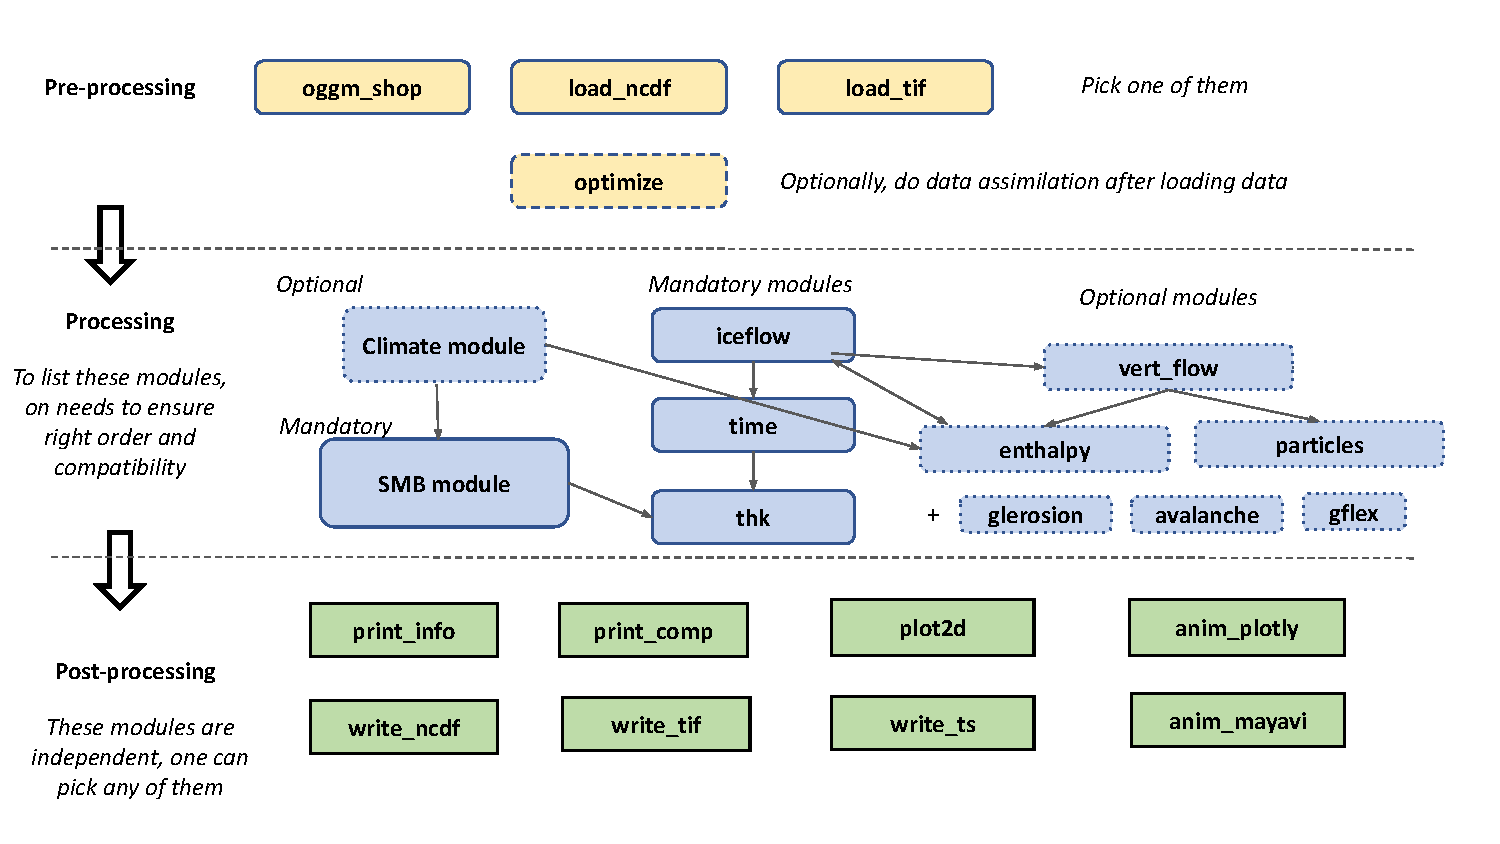
\includegraphics[width=\textwidth]{fig/IGM-modules-flowchart.pdf}
\caption{Flowchart of IGM modules.}
\label{flowchart}
\end{center}
\end{figure*}

In the following sections, we describe the most important 
IGM modules, each identified by a keyword.

\subsection{Pre-processing modules}

Pre-processing modules (Fig. \ref{flowchart}) are essentially collecting data (\texttt{oggm\_shop}),
reading data from files (\texttt{load\_ncdf} and \texttt{load\_tif}).
Optionally, a data assimilation step (\texttt{optimize} module) can be incorporated after reading the data.

\subsubsection{\texttt{oggm\_shop}}
\label{module_oggm}

This module utilizes the Open Glacier Global Model \citep[OGGM][]{maussion2019open} 
(and then depends on python package \texttt{oggm}) to acquire data for runnin the inverse 
and forward glacier evolution model for present-day glaciers.
Users provide the RGI ID (parameter \texttt{oggm\_RGI\_ID})
of the glacier they are interested in, typically obtained from sources such as
\url{https://www.glims.org/maps/glims}).
The data provided by OGGM is preprocessed with a spatial resolution of 100 m and a 
oggm\_border size of 30 m, and available on servers. 
However, users can customize the spatial resolution and oggm\_border
size by setting parameter \texttt{oggm\_preprocess} to \texttt{False}, and setting \texttt{oggm\_dx} 
and \texttt{oggm\_border} parameters to desired values.
Upon running this module, its automatically downloads an ensemble of data related to the 
specified glacier, which is then stored in a folder named after the RGI ID. 
Users can select 2D gridded variables of interest from the available products 
(see Table \ref{oggm_products}). These selected variables are transformed into TensorFlow 
objects, making them accessible within the code as an attribute to the \texttt{state} variable, 
e.g. \texttt{state.thk} designes the ice thickness array, and \texttt{state.thk} designes the basal 
topgraphy. In addition, the module may also download available ice thickness profile data 
\citep{GlaThiDa}, and rasterize the data on the working grid into variable
\texttt{state.thkobs} (referrring to observed thickness), which is filled with NaN values
where no measurements are available.
A copy of the selected variables is stored in a NetCDF file, which can be
run using the \texttt{load\_ncdf} module, eliminating the need to re-download the data.



\begin{table}
\begin{tabular}{|c|c|}
\hline 
Variable & Reference \\ 
\hline 
Surface DEM   & Copernicus DEM GLO-90 \\ 
Ice thickness & \citep{millan2022ice} \\ 
Ice thickness & \citep{farinotti2019consensus} \\ 
Surface ice speeds & \citep{millan2022ice} \\ 
Surface ice speeds & \url{its-live.jpl.nasa.gov} \\ 
Glacier mask & Randolph Glacier Inventory  \\ 
Ice thickness profile & \citep{GlaThiDa} \\
Glacier change & \citep{hugonnet2021accelerated} \\
Climate data & GSWP3\_W5E5 \\
Flowline & OGGM \\
\hline 
\end{tabular} 
$ $ \\ $ $ \\
\caption{Products available with the \texttt{oggm\_shop} module. \label{oggm_products} }
\end{table}
 
\subsubsection{\texttt{load\_ncdf} and \texttt{load\_tif}}
\label{module_loads}

The \texttt{load\_ncdf} module is responsible for loading spatial 2D raster data from a 
NetCDF file specified by the \texttt{lncd\_input\_file} parameter. It transforms all existing 2D fields within 
the NetCDF file into TensorFlow variables, which become attributes of the \texttt{state} object.
The module is expected to import at least the basal topography, which is represented by
the variable \texttt{state.topg}. Optionally, it can provide other fields such as the 
initial ice thickness \texttt{state.thk} and more. Any field present in the NetCDF file 
will be passed as TensorFlow variables, making them accessible as \texttt{state.field}. 
For example, a variable like \texttt{state.icemask} can be provided to delimit the 
accumulation area in the surface mass balance computation and prevent overflowing 
into neighboring catchments.
During this stage, raster data can be resampled or coarsened by a certain factor using 
the \texttt{lncd\_coarsen} parameter. Additionally, it can be cropped to a specific area 
using the \texttt{lncd\_crop} parameter, enabling quicker low-resolution runs or simulations 
in specific regions.
The \texttt{load\_tif} module essentially performs the same task as \texttt{load\_ncdf}, 
but it reads all tif files (e.g., \texttt{topg.tif}) found in the working directory 
and transforms them into TensorFlow variables, named after the file name.


\subsubsection{\texttt{optimize}}
\label{module_optimize}

The module \texttt{optimize} implements the inverse modelling described in Section \ref{inv_model}.
Solving the optimization problem greatly leverages the automatic differentiation tools provided by the
Tensorflow library, and the description of the ice flow model as a neural network (Section \ref{module_iceflow}). 
We refer to \citet{jouvet2023inversion} for a detailed explanation of the methodology.
Here, we will describe how to use the \texttt{optimize} module for data assimilation as a preliminary step 
to a forward or prognostic model run.
Note that his module was designed for isothermal ice without additional \texttt{enthalpy} module.

Before running the module, it is crucial to gather as much observational data as possible. 
This can be done using \texttt{oggm\_shop} module (Tab. \ref{oggm_products}) or reading 
these data from data file with \texttt{load\_ncdf} and \texttt{load\_tif}. 

Observational data follows a convention where variable names end with \texttt{obs}.
Once optimized, the resulting variables are named according to the convention,
but without the additional \texttt{obs} suffix.
Typically, we may use observed horizontal ice surface ice velocities ${\bf u}^{s,obs}$,
(named as \texttt{uvelsurfobs} and \texttt{vvelsurfobs}), top surface elevation $s^{obs}$,
(\texttt{usurf}), ice thickness profiles $h_p^{obs}$ (\texttt{thkobs}), 
glacier mask from RGI outlines (\texttt{icemask}) to enforce zero ice thickness outside the mask,
and (\texttt{thkinit}) a formerly-inferred ice thickness field to initalize the inverse model 
(Tab. \ref{oggm_products}).
All the observational data (including individual ice thickness profiles) are rasterized on the same grid. 
Pixels that do not contain data are ignored in the optimization, 
typically represented by NaN (not-a-number) values.

While the optimization problem is presented in its most general form (Section \ref{inv_model}), 
the user can select a sub-ensemble of controls and 
constraints within the cost function based on the availability of data.
Parameter \texttt{opti\_control} defines the list of variables to optimize 
(e.g. \texttt{['thk','slidingco','usurf']}),
while parameter \texttt{opti\_cost} defines the list of cost components to minimize
(e.g. \texttt{['velsurf','thk','usurf','icemask']}). 

Finding a balance between controls and constraints is crucial to maintaining the 
well-posedness of the problem and guarding against multiple solutions. It is advisable 
to begin with a simple optimization approach, starting with just a single control
(typically \texttt{thk}), and a few target/cost component (typically \texttt{velsurf},
and \texttt{icemask}). Once the simple optimization gives meaningfull results,
the complexity of the optimization can be increased by adding controls and cost components. 
There are a couple parameters that may need tuning for each application:
\begin{itemize}
\item Confidence levels (i.e. tolerance to fit the data) $\sigma^u, \sigma^h, \sigma^s, \sigma^d$ 
may be changed to fit surface ice velocity, ice thickness, surface top elevation, or divergence 
of the flux by changing parameters \texttt{opti\_velsurfobs\_std}, \texttt{opti\_thkobs\_std},
\texttt{opti\_usurfobs\_std}, and \texttt{opti\_divfluxobs\_std}. 
\item Regularization parameters $\alpha^h, \alpha^c$ control the regularization weights 
for the ice thickness $h$ and sliding coefficient $c$ (increasing $\alpha^h, \alpha^c$ 
will make these fields spatially smoother). They can be changed throught parameters 
\texttt{opti\_regu\_param\_thk} and \texttt{opti\_regu\_param\_slidingco}.
\item Parameters $\beta$ and $\gamma$ involved for regularizing the ice thickness $h$
can be changed with parameters \texttt{opti\_smooth\_anisotropy\_factor} 
and \texttt{opti\_convexity\_weight}.
Setting $\beta$ to 1 enforces isotropic smoothing, while reducing $\beta$ increases anisotropy, 
promoting more smoothing along ice flow directions rather than across them. 
This behavior is motivated by expectations for the topography of a glacier bedrock, 
which has undergone long-term erosion.
Adjusting the parameter $\gamma$ to a lower value can be beneficial to improve
the convexity into the system. This can be particularly useful when initializing 
the inverse model with zero thickness or when dealing with margin regions that lack of data.
\end{itemize}

The data assimilation scoring can be monitored during the inverse modelling in several ways:
checking the decrease of misfit cost component, or monitoring the Root-Mean Square Errors between
modelled and observation fields as well as the spatial distribution of these fields.
 
\subsection{Processing modules}

Processing modules implement update rules for all modeled variables within the time loop. 
Most modules correspond to specific physical components. 
For instance, the \texttt{iceflow} module updates 3D ice velocity, 
the \texttt{thk} module handles updates to ice thickness, and so on.
Processing modules must be listed in order: for instance, \texttt{iceflow} must come
before \texttt{thk} as the latter needs the first.

\subsubsection{Climate modules}
\label{module_climate}

Climate modules implement climate forcing in IGM to be used to force the surface 
mass balance or enthalpy models. They output distributed field
of air temperature (variable \texttt{air\_temp} in $^{\circ}$C), 
precipitation (variable \texttt{precipitation} in $kg\,  m^{-2} \, y^{-1}$),
air temperature variablity (variable \texttt{air\_temp\_std} in $^{\circ}$C)
at a given time resolution (e.g. daily, weekly or montly).
Among them, module \texttt{clim\_oggm} reads monthly time series of historical GSWP3\_W5E5 
climate data collected by the \texttt{oggm\_shop} module, and generates monthly 2D 
raster fields of corrected precipitation, mean temperature, and temperature variability.
To achieve this, we first apply a multiplicative correction factor for precipitation
(parameter \texttt{prcp\_fac}) and a biais correction for temperature (parameter \texttt{temp\_bias}).
Then, the module extrapolates temperature data to the entire glacier surface using a reference
height and a constant lapse rate (parameter \texttt{temp\_default\_gradient}). 
In constrast, the point-wise data for precipitation and temperature variablity 
are extended to the entire domain without further correction. 
Module \texttt{oggm\_shop} provides all calibrated parameters.
Module \texttt{clim\_oggm} can addionally generate climate outside the time 
frame of available data as necessary for future scenario-based simulations.
To that aim, we define a reference period with parameter \texttt{clim\_oggm\_ref\_period} 
to pick randomly years within this time interval (usually taken to be a climate-neutral period), 
and apply a biais in temperature and a scaling of precipitation defined by parameter
\texttt{clim\_oggm\_clim\_trend\_array}.
 
\subsubsection{Surface mass balance modules}
\label{module_smb}

These modules provide a rule to update the climatic surface climate mass balance
(variable \texttt{smb}). Here we review two of these models, one computing 
the surface mass balance directly from given parameters, and one from climatic 
variables (Section \ref{module_climate}).
 
Module \texttt{smb\_simple} implements the ``simple'' surface mass balance model
defined by \eqref{smb1}-\eqref{smb2}. To that aim, the four parameters 
$z_{ELA}$, $\beta_{abl}$, $\beta_{acc}$, $m_{acc}$ are given in the
array parameter \texttt{smb\_simple\_array} for some times
(alternatively, these parameters can be provided in an external file).
Then, at time $t$, the module interpolates linearly the four parameters 
from those given in \texttt{smb\_simple\_array}.
 
Module \texttt{smb\_oggm} implements a monthly temperature index model calibrated 
on geodetic mass balance data \citep{hugonnet2021accelerated} by OGGM \citep{maussion2019open}.
The yearly surface mass balance at any point is computed with \eqref{smb3} from 
monthly temperature and precipitation fields as described in Section \ref{module_climate}. 
 
\subsubsection{\texttt{iceflow}}
\label{module_iceflow}

This module models ice flow dynamics in 3D using a Convolutional Neural Network 
(CNN, Fig. \ref{mapping-illu})
based on Physics Informed Neural Network as described by \citet{jouvet2023ice}. 
Our CNN predicts horizontal ice flow $({\bf u}_H, {\bf v}_H)$ from input fields 
which includes ice thickness $h_H$, surface topography $s_H$, ice flow parameters $A_H$ 
and sliding coefficient $c_H$, and spatial grid resolution $H_H$ (Fig. \ref{mapping-illu}). 
The CNN is trained to minimize the energy associated with the Blatter-Pattyn 
ice flow model (as described in Section \ref{phys_ice_dynamics}), 
during the time iterations of a glacier evolution model. This energy reads
\begin{align}
\mathcal{J} ({\bf v}) & =
\int_{V} 2 \frac{A^{-\frac{1}{n}}}{1+\frac{1}{n}} |  D ({\bf v}) |^{1+\frac{1}{n}}  dV  
+  \int_{\Gamma} \frac{c}{1+m}  |{\bf v}|^{1+m}_M   dS  \nonumber \\
& +  \rho g \int_{V} ( \nabla s \cdot {\bf v} ) dV
- \int_{\partial \Omega} {\bf F}(h) \cdot {\bf v}  dS,
\label{functional}
\end{align}
where $V$ and $\Gamma$ denote the ice volume and bedrock interface, respectively \citep{jouvet2023ice}.
This approach offers a computationally-efficient alternative to traditional solvers and exhibits the capability 
to handle a variety of ice flow regimes, along with the ability to memorize previous solutions.
In the IGM strategy, we initially load a pretrained iceflow emulator provided with the IGM package. 
Subsequently, we retrain the iceflow emulator regularly within 
the time loop to maintain its accuracy, ensuring fidelity to the solver, and adapting 
it to updated glacier geometries. As retraining costs about 3 times more than a CNN evaluation,
we strive to minimize the frequency of retraining \citep{jouvet2023ice}. 

\begin{figure}[!ht]
\begin{center}
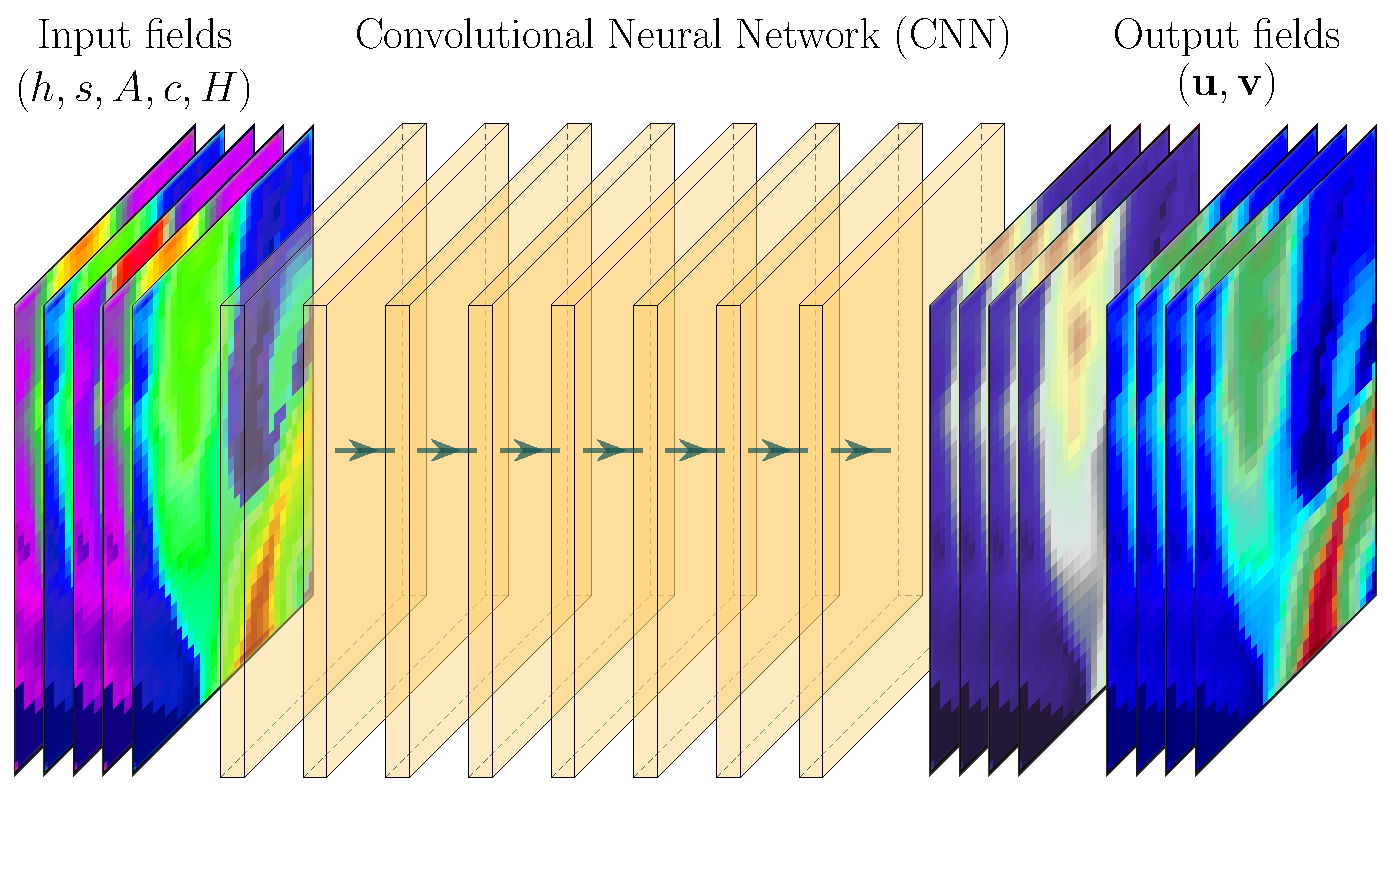
\includegraphics[width=0.48\textwidth]{fig/mapping-illu7.pdf}
\caption{\label{mapping-illu} Our iceflow emulator consists of a CNN that maps 
geometrical (thickness and surface topography), ice flow parameters 
(shearing and basal sliding), and spatial resolution inputs to 3D ice flow fields.}
\end{center}
\end{figure}

Parameters associated with this module are of several kinds:
\begin{itemize}
\item Physical parameters includes Glen's exponent $n$ (\texttt{iflo\_exp\_glen}), Weertman's exponent $m$
(\texttt{iflo\_exp\_weertman}), initial sliding coefficient $c$ (\texttt{iflo\_init\_slidingco}) 
and initial arrhenius factor $A$ (\texttt{iflo\_init\_arrhenius}) defined in Section \ref{phys_ice_dynamics}.
Note that $A$ and $c$ are automatically updated when using module \texttt{enthalpy}.
\item Parameters associated with vertical discretization include the number of points $N_z$ 
along the vertical direction (\texttt{iflo\_Nz}) and the parameter 
\texttt{iflo\_vert\_spacing}, which controls the density of points near the bedrock. 
By default, \texttt{iflo\_vert\_spacing} is set to 4. This means that the layers are 
distributed according to a quadratic rule, resulting in four times finer 
discretization near the ice-bedrock interface, where the steepest gradients are expected, 
compared to the discretization near the ice surface.
\item Parameter \texttt{iflo\_retrain\_emulator\_lr} controls the learning rate for the retraining
of the CNN: A low number results in a gentle learning with the downside that several iterations
may be needed to achieve optimal learning. On the other hand, \texttt{iflo\_retrain\_emulator\_freq} 
controls the retraining frequency, which needs to be sufficiently frequent to maintain accuracy,
but not too much to mitigate computational costs.
When treating large arrays, retraining must be done sequentially patch-wise for memory reason. 
The maximum size of patches is controlled by parameter \texttt{iflo\_multiple\_window\_size}.
\item One can choose between using the iceflow emulator (the default choice, achieved 
by setting \texttt{iflo\_type} to \texttt{emulated}), the solver (set \texttt{iflo\_type} 
to \texttt{solved}), or both (set \texttt{iflo\_type} to \texttt{diagnostic})
to assess the fidelity of the iceflow emulator to the solver.
\item One may choose between 2D Arrhenius factor (allowing horizontal variations only)
by changing parameters between \texttt{iflo\_dim\_arrhenius} to 2 or 3. 
Turning it to 3 is necessary for the enthalpy model.
\end{itemize}

\subsubsection{\texttt{time}}
\label{module_time}

This module computes the time step with the following criteria:
i) It is adjusted precisely to allow matching with specified saving times, 
whose the frquency is defined by parameter \texttt{time\_save}.
ii) It remains below a designated maximum time step, 
as determined by the parameter \texttt{time\_step\_max}.
iii) It complies to the Courant-Friedrichs-Lewy (CFL) condition, as governed by 
the parameter \texttt{time\_cfl}.
Indeed, to ensure stability in the transport scheme for ice thickness evolution, 
it is essential that the time step respects the CFL condition.
The module additionally updates the time \texttt{time} in addition to the time step 
\texttt{time}. Other key parameters of this module are \texttt{time\_start} 
and \texttt{time\_end}, which define the simulation starting and ending times.

\subsubsection{\texttt{thk}}
\label{module_thk}

This module solves the mass conservation equation \eqref{conservationeq} to update ice 
thickness based on the results obtained from the \texttt{iceflow} module and the 
surface mass balance computed by another module. Equation 
\eqref{conservationeq} is solved using an explicit first-order upwind finite-volume 
scheme on the 2D working grid.
In this scheme, ice mass is permitted to move between adjacent cells where thickness 
and velocities are defined. This movement is determined by edge-defined fluxes, 
which are inferred from depth-averaged velocities and ice thickness in the upwind direction. 
The resulting scheme is both mass-conserving and parallelizable, 
thanks to its fully explicit nature. However, it is subject to a Courant-Friedrichs-Lewy 
(CFL) condition, as explained in the previous section. This condition guarantees 
that no more than the entire content of one cell is transferred to a neighboring cell 
within a single iteration.

\subsubsection{\texttt{vert\_flow}}
\label{module_vertical}

Since the \texttt{iceflow} module is based on the Blatter-Pattyn ice flow model and 
predicts only the horizontal components of ice velocity, an additional module, 
\texttt{vert\_flow} is responsible for computing the vertical component, 
denoted as \texttt{state.W}, using the horizontal components \texttt{state.U} 
computed by the \texttt{iceflow} module. 
This computation is achieved by integrating the incompressibility condition \eqref{eq_incomp}.
The \texttt{vert\_flow} module is mandatory in various other modules, 
such as \texttt{particle} which involves 3D particle trajectory integration, and the 
\texttt{enthalpy} module, which is responsible for computing the 3D advection-diffusion of enthalpy.

\subsubsection{\texttt{enthalpy}}
\label{module_enthalpy}

The \texttt{enthalpy} module is responsible for updating the 3D enthalpy field based 
on the mechanical state by solving the advection-diffusion equation \eqref{enth1}-\eqref{enth2}. 
This process includes applying the top and bottom boundary conditions described in Section
\ref{phys_enthalpy}.
To achieve this, the variable $E$ (and equivalently, $T$ and $\omega$) is defined 
on the same 3D structured grid than the ice flow field $\mathbf{u}$. 
Solving equations \eqref{enth1}-\eqref{enth2} is done in two steps through time splitting operators.
First, an explicit first-order upwind finite-volume scheme is employed to solve the 
advective component in the horizontal direction, following a similar scheme as the one 
used in the mass conservation equation:
\begin{align}
 E^{n+\frac12}  = E^n - dt \left( u^n_x \frac{\partial E^n}{ \partial x} 
  + u^n_y \frac{\partial E^n}{ \partial y} \right),
\label{E_step1}
\end{align}
In a second time we solve the remaining advection-diffusion equation with respect to the 
vertical direction in an implicit manner:
\begin{align}
& \rho_i \left( \frac{E^{n+1}-E^{n+\frac12}}{ dt}
+ u_z \frac{\partial E^{n+1}}{ \partial z} \right) \\
& - \frac{\partial }{\partial z} \left(
K_{c,t} \frac{\partial E^{n+1}}{ \partial z} \right) 
 = \phi^n - \rho_w L D_w(\omega^{n+\frac12}).
\label{E_step2}
\end{align}

This is done by finite differences, where the advection term is approximated using 
an upwind method, while the diffusion term is approximated using a centered scheme. 
Once the top and bottom boundary conditions are incorporated, the discretization leads 
to solving $N_y \times N_x$ tridiagonal systems, each with 
a size equal to the number of layers $N_z$. Solving these tridiagonal 
systems is accomplished using the tridiagonal matrix algorithm (or Thomas algorithm). 
This algorithm requires approximately $3 \times N_z$ operations per column, 
translating to a total of $3 \times N_z \times N_y \times N_x$ operations in total.
Tensorflow ensures  parallelism of operations between column-wise problems. 
Following solving the enthalpy equation, the process involves computing the basal 
melt rate using \eqref{basal_melt_rate}, updating it along with the enthalpy to account 
for water drainage along the ice column.
This step also calculates the resulting water thickness from \eqref{W_till} and 
sliding coefficient from \eqref{sliding_param}.

In summary, assuming known enthalpy $E^n$, ice thickness geometry $h^{n+1}$, iceflow ${\bf u}^{n+1}$,
vertical ice flow $u^{n+1}_z$, updating the enthalpy at time $t^{n+1}$ requires to perform the following sub-steps:
\begin{itemize}
\item Compute the mean surface temperature $T^n_s$ to enforce the upper surface Dirichlet 
boundary condition. This temperature is capped at 0$^{\circ}$C to maintain the temperature 
of ice below pressure-melting point.
\item Compute the vertical discretization with the new ice geometry $h^{n+1}$.
\item Compute the temperature $T_{pmp}^n$ and enthalpy $E_{pmp}^n$ at pressure melting point
using \eqref{Tpmp}.
\item Compute the ice temperature $T^n$ from the enthalpy $E^n$ using \eqref{def_enth}.
\item Compute the Arrhenius factor $A(T^n)$ from temperature $T^n$ using \eqref{A1}-\eqref{A2}.
\item Compute the 3D strain heat $\phi^{n+1}$ from ice flow field ${\bf u}^{n+1}$ 
and Arrhenius factor $A(T^n)$ using \eqref{def_phi}.
\item Compute the 2D basal frictional heat $Q_{\rm fh}^{n+1}$, from basal velocity field 
${\bf u}^{n+1}$ and sliding coefficient $c^n$ using \eqref{def_Q}.
\item Compute the surface enthalpy $E^n_s$ from the surface temperature $T^n_s$
 using \eqref{def_enth}.
\item Compute the updated enthalpy $E^{n+\frac12}$ after solving one explicit step for 
the horizonal advection (Eq. \eqref{E_step1}).
\item Compute the updated enthalpy $E^{n+1}$ field solving the 
advection-diffusion equation (Eq. \eqref{E_step2}).
\item Compute the basal melt rate from \eqref{basal_melt_rate}.
\item Compute the water thickness in the till $W^{n+1}$ solving \eqref{W_till} explicity.
\item Compute the sliding parametrization $c^{n+1}$ using \eqref{sliding_param}.
\end{itemize}

\subsubsection{\texttt{particles}}
\label{module_particles}

This module implements a particle tracking routine designed to calculate the time-space 
trajectory of virtual tracers that are advected by the ice flow, representing materials 
like debris or moraines. Thanks to TensorFlow's GPU implementation, a substantial number 
of particles can be efficiently computed in parallel. The routine encompasses particle seeding
(the default seeds in the accumulation area at regular intervals), and particle tracking, 
achieved through advection using the 3D velocity field. 
For that purpose, one uses a simple explicit forward-in-time Euler scheme. 
The positions of particles are stored within vectors of length equal to the number of tracked 
particles: \texttt{state.xpos}, \texttt{state.ypos}, and \texttt{state.zpos}.
There is currently no strategy in place for removing particles. 
Presently, there are two implementations available, controlled 
by the parameter \texttt{part\_tracking\_method}:
\begin{itemize}
\item \texttt{simple}: 
In the horizontal plane, particles are advected using the horizontal velocity field, 
with interpolation performed bilinearly.
In the vertical direction, particles are tracked along the ice column, scaling their 
position between 0 and 1, where 0 represents the bed and 1 corresponds to the top surface. 
The evolution of the particles within the ice column over time is determined by the surface 
mass balance: when the surface mass balance is positive (indicating ice accumulation), 
the particles move deeper within the ice column, reducing their relative height. 
Conversely, when the surface mass balance is negative (indicating ice ablation), 
the particles rise within the ice column, increasing their relative height.
\item \texttt{3d}: This method advects particles from the the 3D ice flow velocity field. 
Unlike the ``simple'' method, one needs to access the vertical ice velocity component
by activating \texttt{vert\_flow} module.
\end{itemize}
The seeding strategy is flexible and can be easily modified. To that aim, 
one simply needs to redefine the function \texttt{igm.seeding()} in a file \texttt{particles.py}.
Note that particles can be plotted with \texttt{plot2d} module, or being written 
in a separate file.

\subsection{Post-processing modules}

IGM includes post-processing modules that allow for result monitoring. 
The frequency of saving is determined by the parameter \texttt{params.time\_save}, 
which is defined within the \texttt{time} module.

\subsubsection{\texttt{plot2d}}
\label{module_plot2d}

Based on \texttt{matplotlib},
the \texttt{plot2d} module generates 2D plan-view plots (possibly with overlayed particles), 
which can be displayed in real-time or saved as image files. These plots visualize variables 
defined by the parameter \texttt{params.plt2d\_var}, which can be set to any 2D variables as defined
in Tab. \ref{variable_name}.

\subsubsection{\texttt{write\_ncdf} and \texttt{write\_tif}}
\label{module_write}

The \texttt{write\_ncdf} and \texttt{write\_tif} modules are responsible for writing 
2D field variables that are specified in the parameter lists:
\texttt{params.wncd\_vars\_to\_save} and \texttt{params.wtif\_vars\_to\_save}, 
respectively. These variables are written into the NetCDF output file specified by the 
parameter \texttt{params.wncd\_output\_file} and into TIF output files.
For tif files, files are created in the working directory with names composed by the 
variable name and the time (e.g., thk-000040.tif, usurf-000090.tif).
 
\subsubsection{\texttt{anim\_plotly}}
\label{module_plotly}
 
This module permits an interactive 3D vizualization of IGM results reading the NetCDF file
produced by module \texttt{write\_ncdf} based on libraries \texttt{dash} and \texttt{plotly}.
It creates a dash app that can be accessed via a browser
(the adress printed in the console is usually \url{http://127.0.0.1:8050/}). 
The app shows a 3D plot of the glacier's surface on top of the surrounding bedrock. 
The surface color shows either the ice thickness, the velocity magnitude of the surface
or the surface mass balance. Variables can be chosen in the dropdown menu.
The app also includes a slider to navigate the different time steps of the glacier simulation.

\subsubsection{\texttt{anim\_mayavi}}
\label{module_mayavi}

This module based on the \texttt{mayavi} and \texttt{pyqt5} libraries
produces a 3D animated plot using from the 
NetCDF output file produced by module \texttt{write\_ncdf}.

%%%%%%%%%%%%%%%%%%%%%%%%%%%%%%%%%%%%%%%%%%%%%%%%%%%%%%%%%%%%%

\section{Applications} 

\subsection{ISMIP-HOM experiments}

See \citep{jouvet2023ice}

\subsection{Enthalpy experiments}

Following \citep{wang2020two}, we carry the two benchmark experiments proposed by 
\citep{kleiner2015enthalpy} and one from \citep{hewitt2017models} to
verify the implementation of the enthalpy formulation.

Experiment A considers a flat parallel-sided slab with a constant thickness $h$ = 1000 m
without any ice dynamics so that only the vertical heat diffusion is modelled. We perform
a transient simulation during 300'000 years with a constant geothermal heat flux at the base. 
The surface temperatures are prescribed to -30$^{\circ}$C all the time except between
$t=100'000$ years and $t=150'000$ years. Fig. \ref{KleinerExpA} 
shows the time series of the simulated basal temperatures,
basal melt rates, and basal water layer thicknesses. As a result, they compare very well with 
with reference solutions shown in Fig 1 of \citep{kleiner2015enthalpy}. 

\begin{figure}[!h]
\begin{center} 
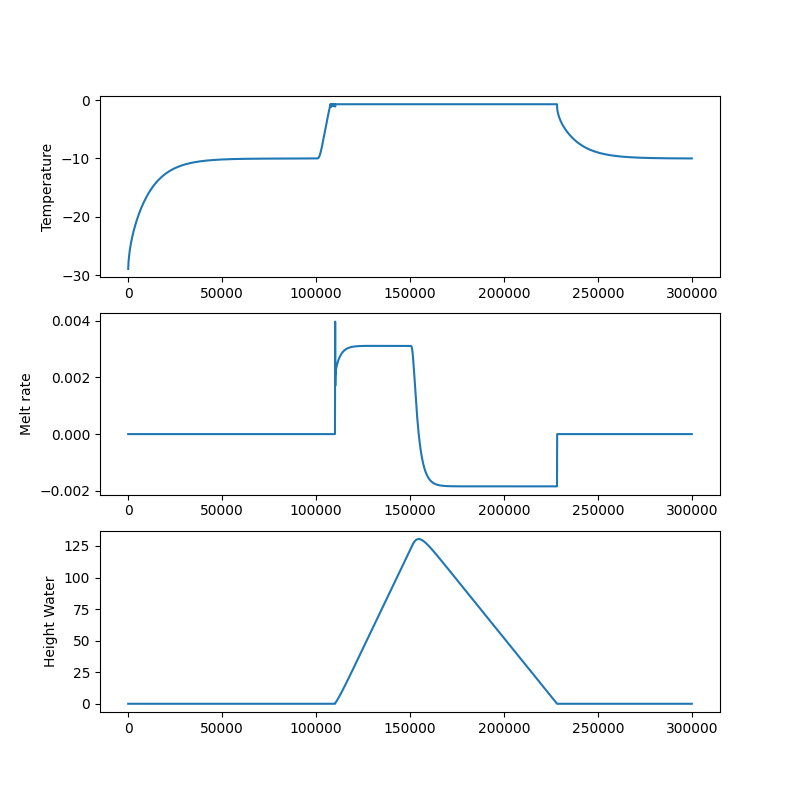
\includegraphics[width=0.48\textwidth]{fig/KleinerExpA.png}   
\end{center}
\caption{ Result of experiment A of \citep{kleiner2015enthalpy}. \label{KleinerExpA}}
\end{figure}

Experiment B also considers a parallel-sided slab but with a constant thickness $h=200$ m
and a slope of 4 $^{\circ}$. The horizontal ice velocity is defined by a SIA-like profile, 
while the vertical ice velocity is constant. 
The enthalpy at the surface is prescribed with -3$^{\circ}$C and zero water content.
We assume zero geothermal heat flux and basal sliding velocity.
Here, only the strain heating acts as heat source. We initialize 
the transient simulation with a constant enthalpy field with -1.5$^{\circ}$C 
and zero water content. We assume the thermal diffusivity of temperate ice to be 
100'000 times lower than the one of the cold ice. We run the simulation until
reaching a steady state, which is after 1000 years.
As a result, they compare well with 
the reference solution shown in Fig 4 of \citep{kleiner2015enthalpy}. 

\begin{figure}[!h]
\begin{center} 
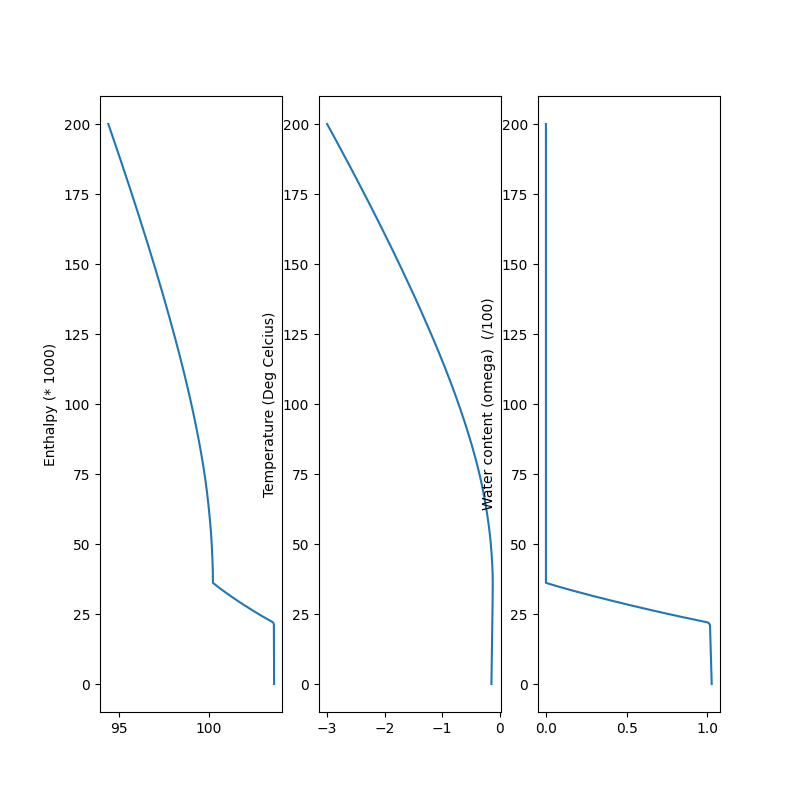
\includegraphics[width=0.48\textwidth]{fig/KleinerExpB.png}   
\end{center}
\caption{ Result of experiment B of \citep{kleiner2015enthalpy}. \label{KleinerExpB}}
\end{figure}

Last, we reproduced the experiment proposed by \citet{hewitt2017models},
which consider an idealized ice cap geometry. Again, the horizontal ice velocity 
and the strain heating are defined based on SIA-like ice flow. We impose 
a constant temperature on the top surface of the ice cap, while we assume 
the bedrock to be at the pressure melting point. The simulation is initialized 
with a constant enthalpy field  with -11$^{\circ}$C and zero water content.
The simulation is run until steady state.
Fig. \eqref{hewitt2017} shows the result at steady-state with a drainage function.
As a result, it compares reasonably with the reference solution shown in Fig 7b 
of \citep{hewitt2017models}. It is likely that a higher number of layers would
imporve the match between the two.

\begin{figure}[!h]
\begin{center} 
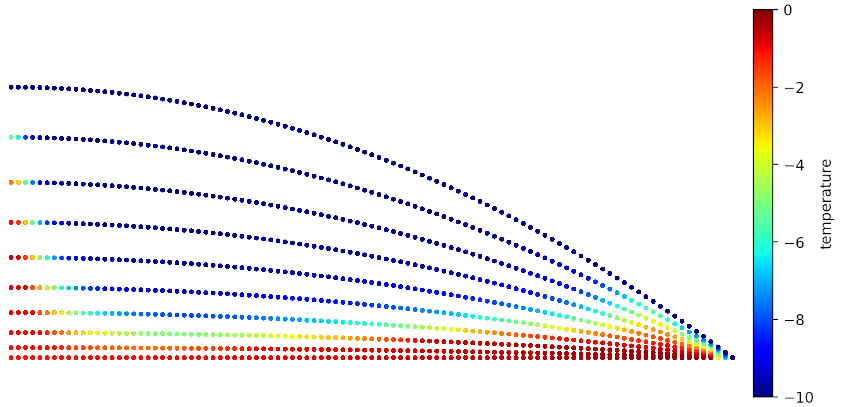
\includegraphics[width=0.48\textwidth]{fig/hewitt2017.png}   
\end{center}
\caption{ Result of the ice cap experiment  of \citep{hewitt2017models}. \label{hewitt2017}}
\end{figure}

%%%%%%%%%%%%%%%%%%%%%%%%%%%%%%%%%%%%%%%%%%%%%%%%%%%%%%%%%%%%%

\bibliographystyle{apalike}
\bibliography{biblio}

\end{document}
